This project will focus on pool tables (pocket billiards). There are many different types of pool such as 8-ball, 9-ball and 14-1. The types differentiate some, but the table and the rest of the equipment is the same.\\

\textbf{Table Specifications:}\\
The international pool regulations concerning table size, cloth colour, ball size and etc. are regulated by "World Pool-Billiard Association"\cite{poolregulations}. These specifications will be used in order to know what size of table, ball etc. that have to be looked for while doing the image processing.

In \ref{fig:partspool} a standard pool table is seen from top view. Different indications of pockets etc. are marked.

\begin{figure}[H]
\begin{center}
\leavevmode
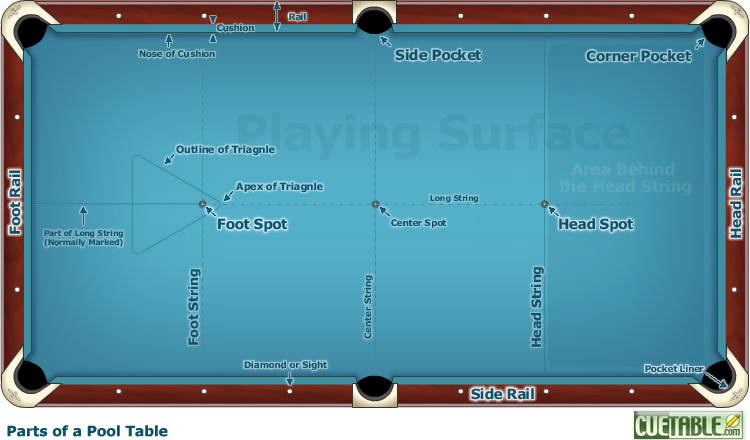
\includegraphics[width=0.9\textwidth]{images/pooltablespecs.jpg}
\end{center}
\caption{Parts of pool table. From cuetable.com}
\label{fig:partspool}
\end{figure}

The rules regulations relevant for the project are listed here:

\begin{itemize}
	\item \textbf{Playing Surface Size:}\\
		Must be rectangular and symmetrical.\\
		9. foot table: 2.54 x 1.27 m.\\
		8. foot table: 2.34 x 1.17 m.\\
	\item \textbf{Rail Size:}\\
		Must be between 10.16 and 19.05 cm including the rubber cushions.\\
	\item \textbf{Diamonds (Sights):}\\
		18 diamonds (or 17 and a name plate) must be attached flush on the rail cap with:\\
		9. foot table: 31.75 cm from diamond to diamond.\\
		8. foot table: 29.20 cm from diamond to diamond.\\
		The center of each diamond must be located 93.5 mm from the nose of the cushion.\\
		The diamonds may be round or diamond-shaped.\\
	\item \textbf{Cloth:}\\
		Only the colors of yellow-green, blue-green or electric blue are acceptable for WPA competition. \\
	\item \textbf{Ball Size:}\\
		All balls should be 5.715 cm in diameter.\\
		A complete set of balls consist of:\\
		Que ball: White\\
		Solid Balls:\\
		\hspace*{10 mm}	1:Yellow, 2:Blue, 3:Red, 4:Purple, 5:Orange, 6:Green, 7: Maroon, 8:Black.\\
		Striped Balls:\\
		\hspace*{10 mm}	9:Yellow, 10:Blue, 11:Red, 12:Purple, 13:Orange, 14:Green, 15:Maroon\\
		
		\begin{figure}[H]
		\begin{center}
		\leavevmode
		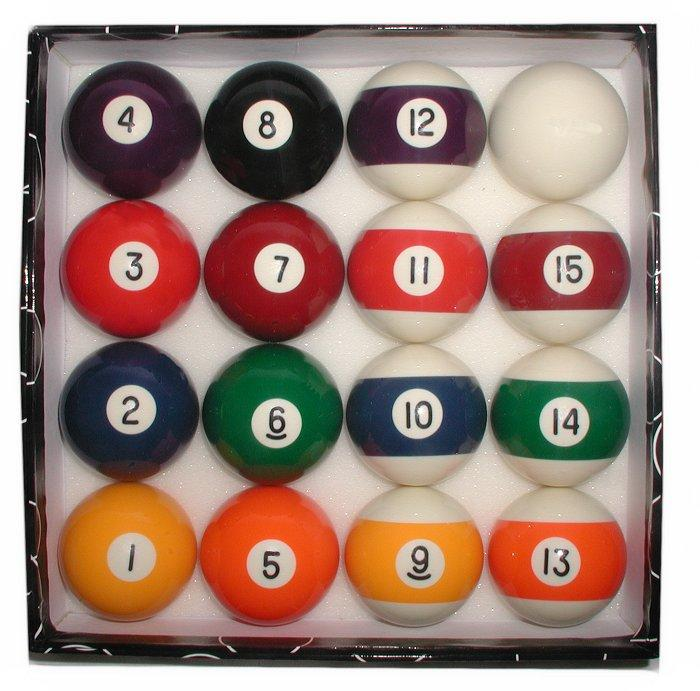
\includegraphics[width=0.4\textwidth]{images/poolballs.jpg}
		\end{center}
		\caption{All the pool balls.}
		\label{fig:poolballs}
		\end{figure}	
		
		
	\item \textbf{Light:}\\
		The bed and rails of the table must receive at least 520 lux. The light should be evenly distributed on the table and the intensity of any directed light on table or player should be non blinding.
\end{itemize}

\textbf{Pool Rules}\\
The rules of pool important for this project will be stated here.

\begin{itemize}
	\item \textbf{Start Position:}\\
		For standard 8- or 9 ball the formation must be set up with the apex ball being on the foot spot. The start position can be seen in \ref{fig:poolstart}.\\
		
\begin{figure}[H]
\begin{center}
\leavevmode
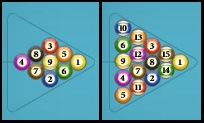
\includegraphics[width=0.4\textwidth]{images/poolstart.jpg}
\end{center}
\caption{Starting position of plays. First image for 9-ball and second for 8-ball.}
\label{fig:poolstart}
\end{figure}

	\item \textbf{Continuing Play:}\\
		The player will remain at the table as long as a legal ball is pocketed or he wins by eventually pocketing the eight ball.\\
		
	\item \textbf{Standard Fouls, Which Gives Cue Ball In Hand To Opponent:}\\
		Cue ball falls of the table.\\
		Hit a non-legal ball first - could be the opponents balls.\\
		Ball falls of table.\\
		
	\item \textbf{Game Finished:}\\
		\textbf{For 8-ball:}\\
		\hspace*{10 mm}Player pockets all legal balls, then 8-ball.\\
		\hspace*{10 mm}Other player pockets 8-ball before all legal balls.\\
		\hspace*{10 mm}Other player drives 8-ball out of play.\\
		\textbf{For 9-ball:}\\
		\hspace*{10 mm}Player pockets all legal balls, then 9-ball.\\
		\hspace*{10 mm}Other player pockets 9-ball before all legal balls.\\
		\hspace*{10 mm}Other player drives 9-ball out of play.\\
\end{itemize}

